\documentclass[12pt]{article} % use larger type; default would be 10pt
\usepackage[utf8]{inputenc} % set input encoding (not needed with XeLaTeX)

%%% PAGE DIMENSIONS
\usepackage{geometry} % to change the page dimensions
\geometry{a4paper} % or letterpaper (US) or a5paper or....
\geometry{margin=2cm} % or letterpaper (US) or a5paper or....

\usepackage{graphicx} % support the \includegraphics command and options
\usepackage[parfill]{parskip} % Activate to begin paragraphs with an empty line rather than an indent
\usepackage{times} % for Times Roman default font

%%% PACKAGES
\usepackage{booktabs} % for much better looking tables
\usepackage{array} % for better arrays (eg matrices) in maths
\usepackage{paralist} % very flexible & customisable lists (eg. enumerate/itemize, etc.)
\usepackage{verbatim} % adds environment for commenting out blocks of text & for better verbatim
\usepackage{subfig} % make it possible to include more than one captioned figure/table in a single float

%%% HEADERS & FOOTERS
\usepackage{fancyhdr} % This should be set AFTER setting up the page geometry
\pagestyle{fancy} % options: empty , plain , fancy
\renewcommand{\headrulewidth}{0pt} % customise the layout...
\lhead{}\chead{}\rhead{}
\lfoot{}\cfoot{\thepage}\rfoot{}

\makeatletter
\renewcommand{\maketitle}{%
  {\bfseries{\scshape{\Large{\@title\par}}}}
}
\makeatother

\hyphenation{Kiwi-bank} % otherwise it may get hyphenated as Ki-wibank

%%% END Article customizations

%%% The "real" document content comes below...

\title{Mt Brown Hut: 14-15 August 2019}

\begin{document}
  \maketitle

We followed the track from Geologist Creek, just passed Dorothy Falls (neither of which are labelled, although the start of the track has a DoC sign).  This begins inocuously enough but becomes quite steep after a kilometre or so.  If I recall correctly the sign indicated a trip of about 4 hours\footnote{We took about 2 hours 40 minutes going up, and 2:20 coming down.}.

We knew Permolat flies coal into this hut, but this is not a practice of which I approve.  Once clear of the bush, we came across quite a bit of freshly cut turpentine scrub (\textit{Dracophyllum uniflorum}) which we collected as we went - carrying it the last fifteen minutes or so to the hut.  This last section was mostly covered in snow.  With my pruning saw, I cut sticks into suitable lengths for the 'Little Cracker' twig burner, and we were gratified to find that, as reputed, this lit and burned readily.

The weather, although nowhere near as bad as it had been, was not particularly good either.  Thus we didn't get the wonderful sunset for which the site is renowned.  However, the sky cleared during the night and we went to bed with great hopes for the morrow.  Unfortunately, it became overcast with low cloud obscuring the peaks by morning.  Thus, we returned the way we had come without exploring the tops.

A nice 4-bunk hut situated in a beautiful spot.  Worth another visit and further exploration of the tops.  However, it is apparently very popular and thus going on weekdays during the shoulder season is probably advisable.

% \begin{figure}[ht]
% % \centering
% \begin{minipage}{.5\linewidth}
% \begin{flushleft}
%    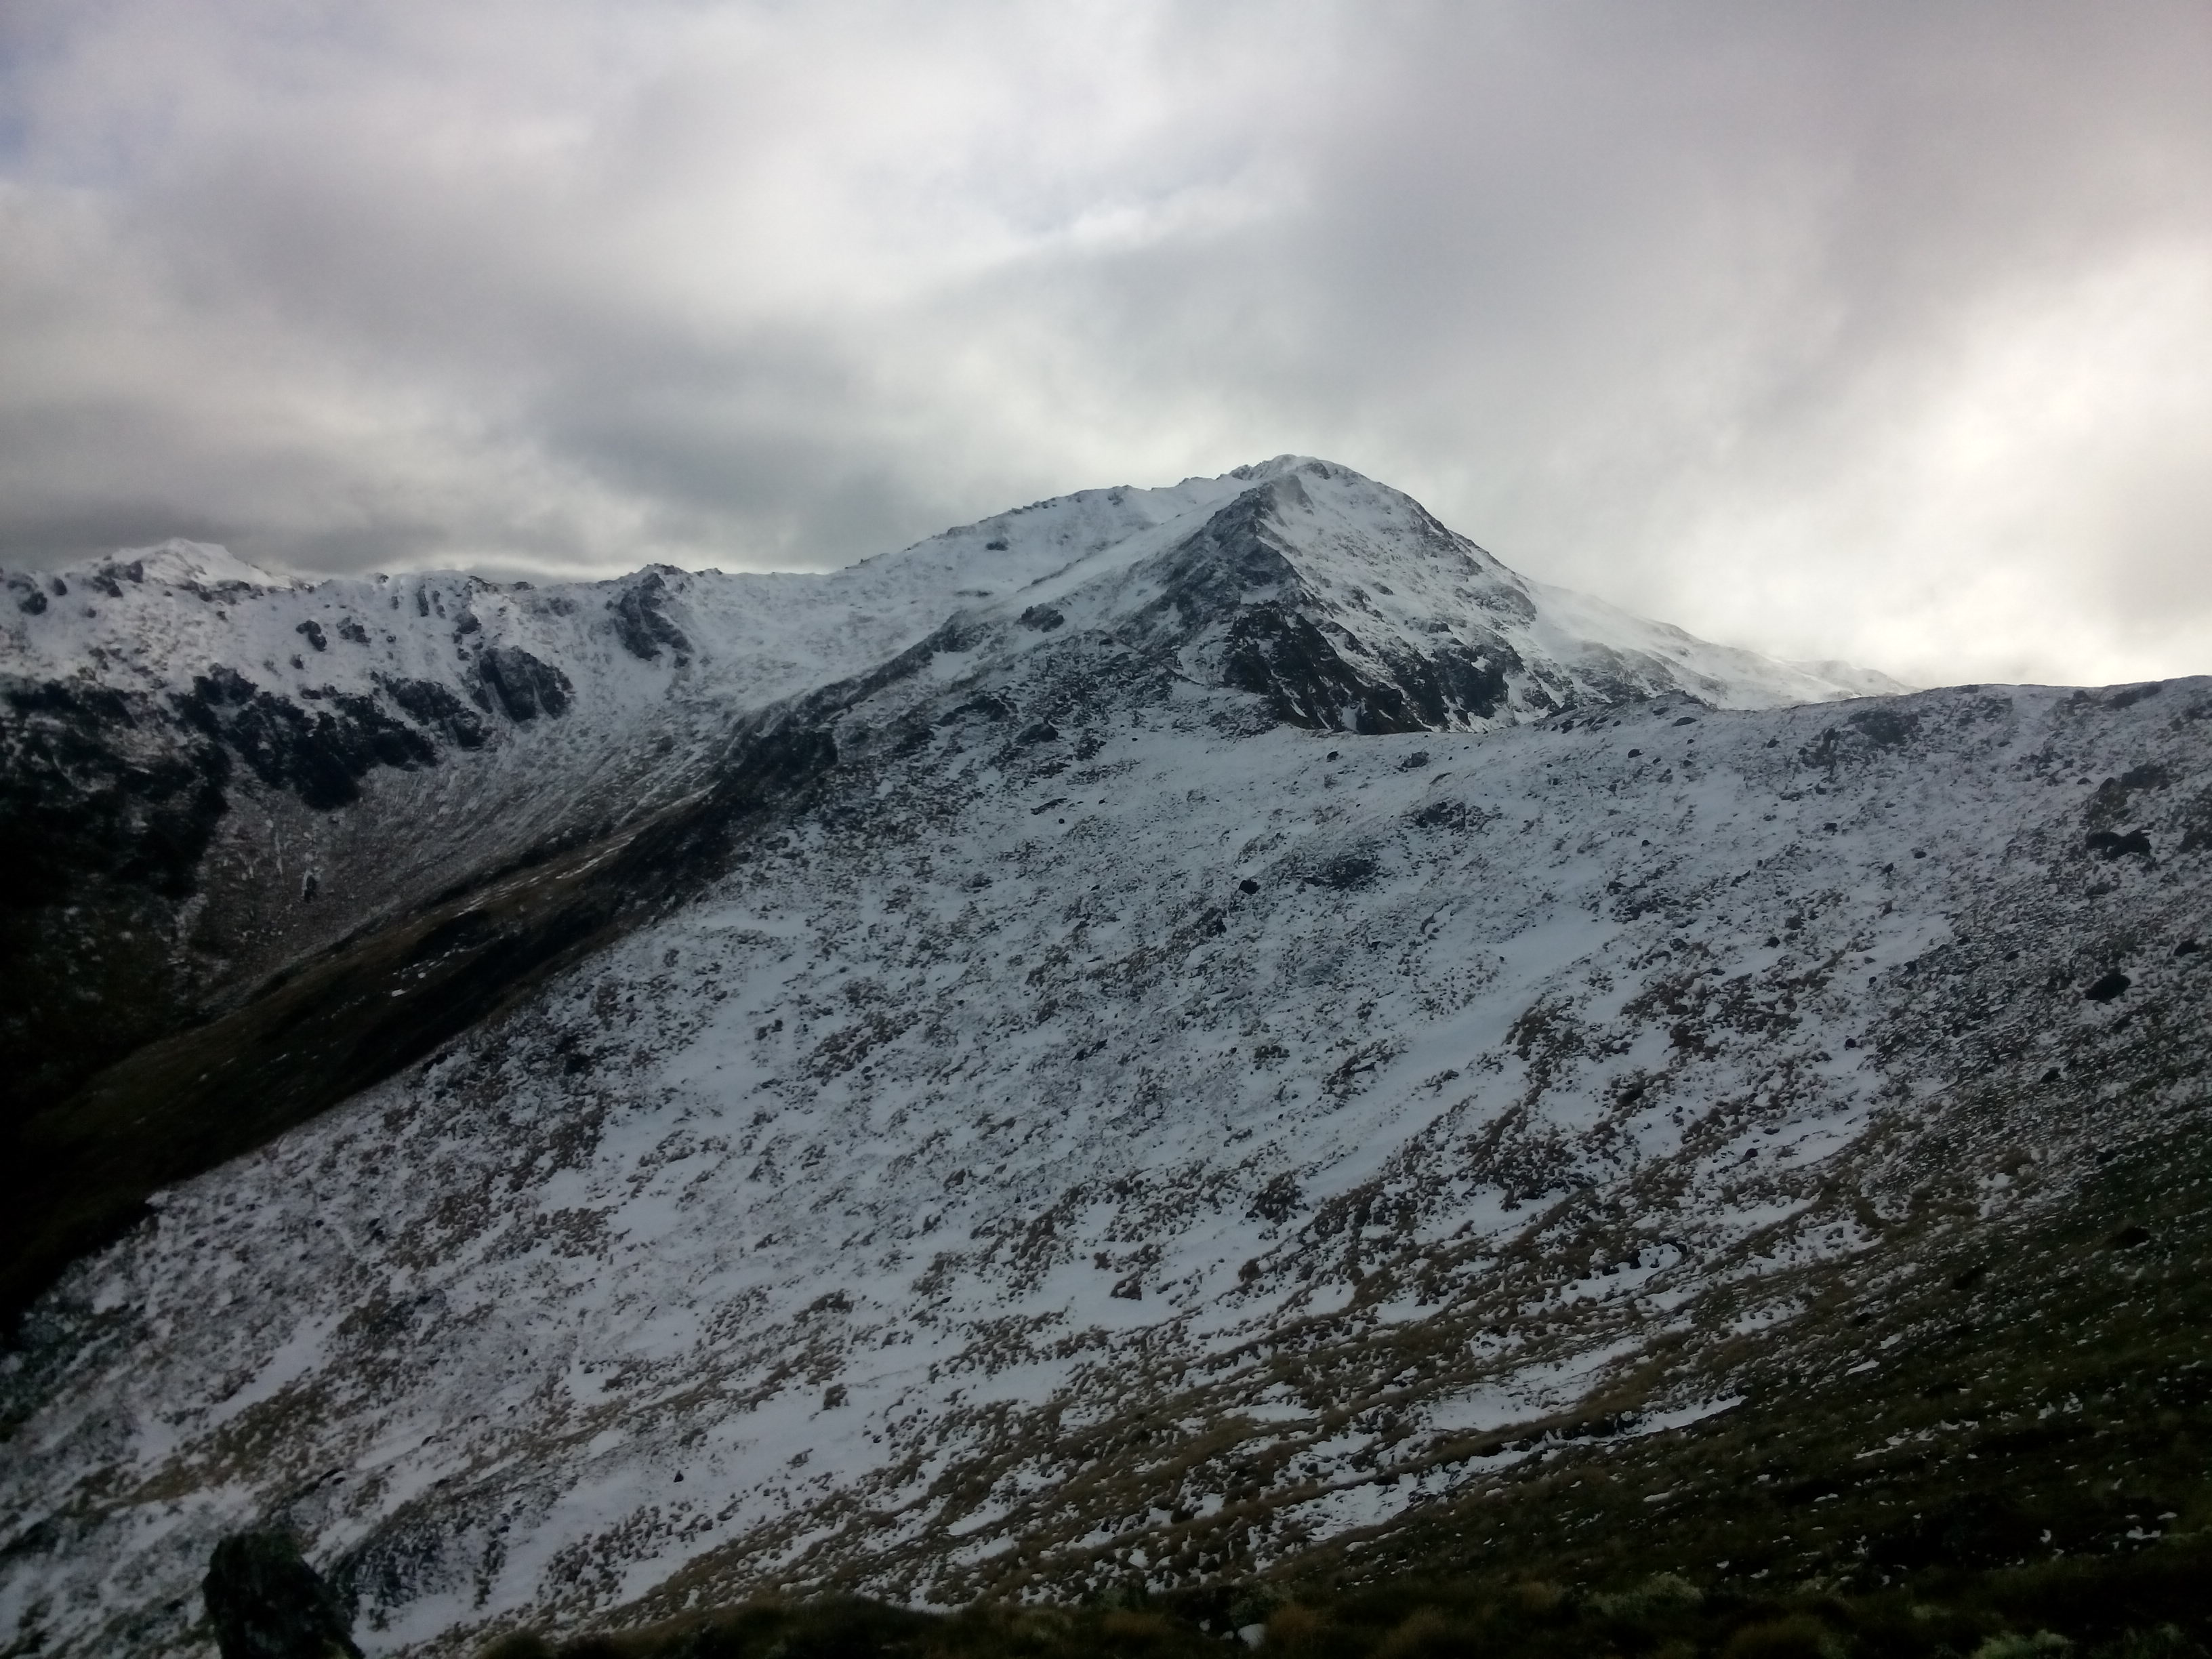
\includegraphics[width=8.5cm]{MtNorma28June2017Photo1}
% \end{flushleft}
% \end{minipage}
% \begin{minipage}{.5\linewidth}
% \begin{flushright}
%     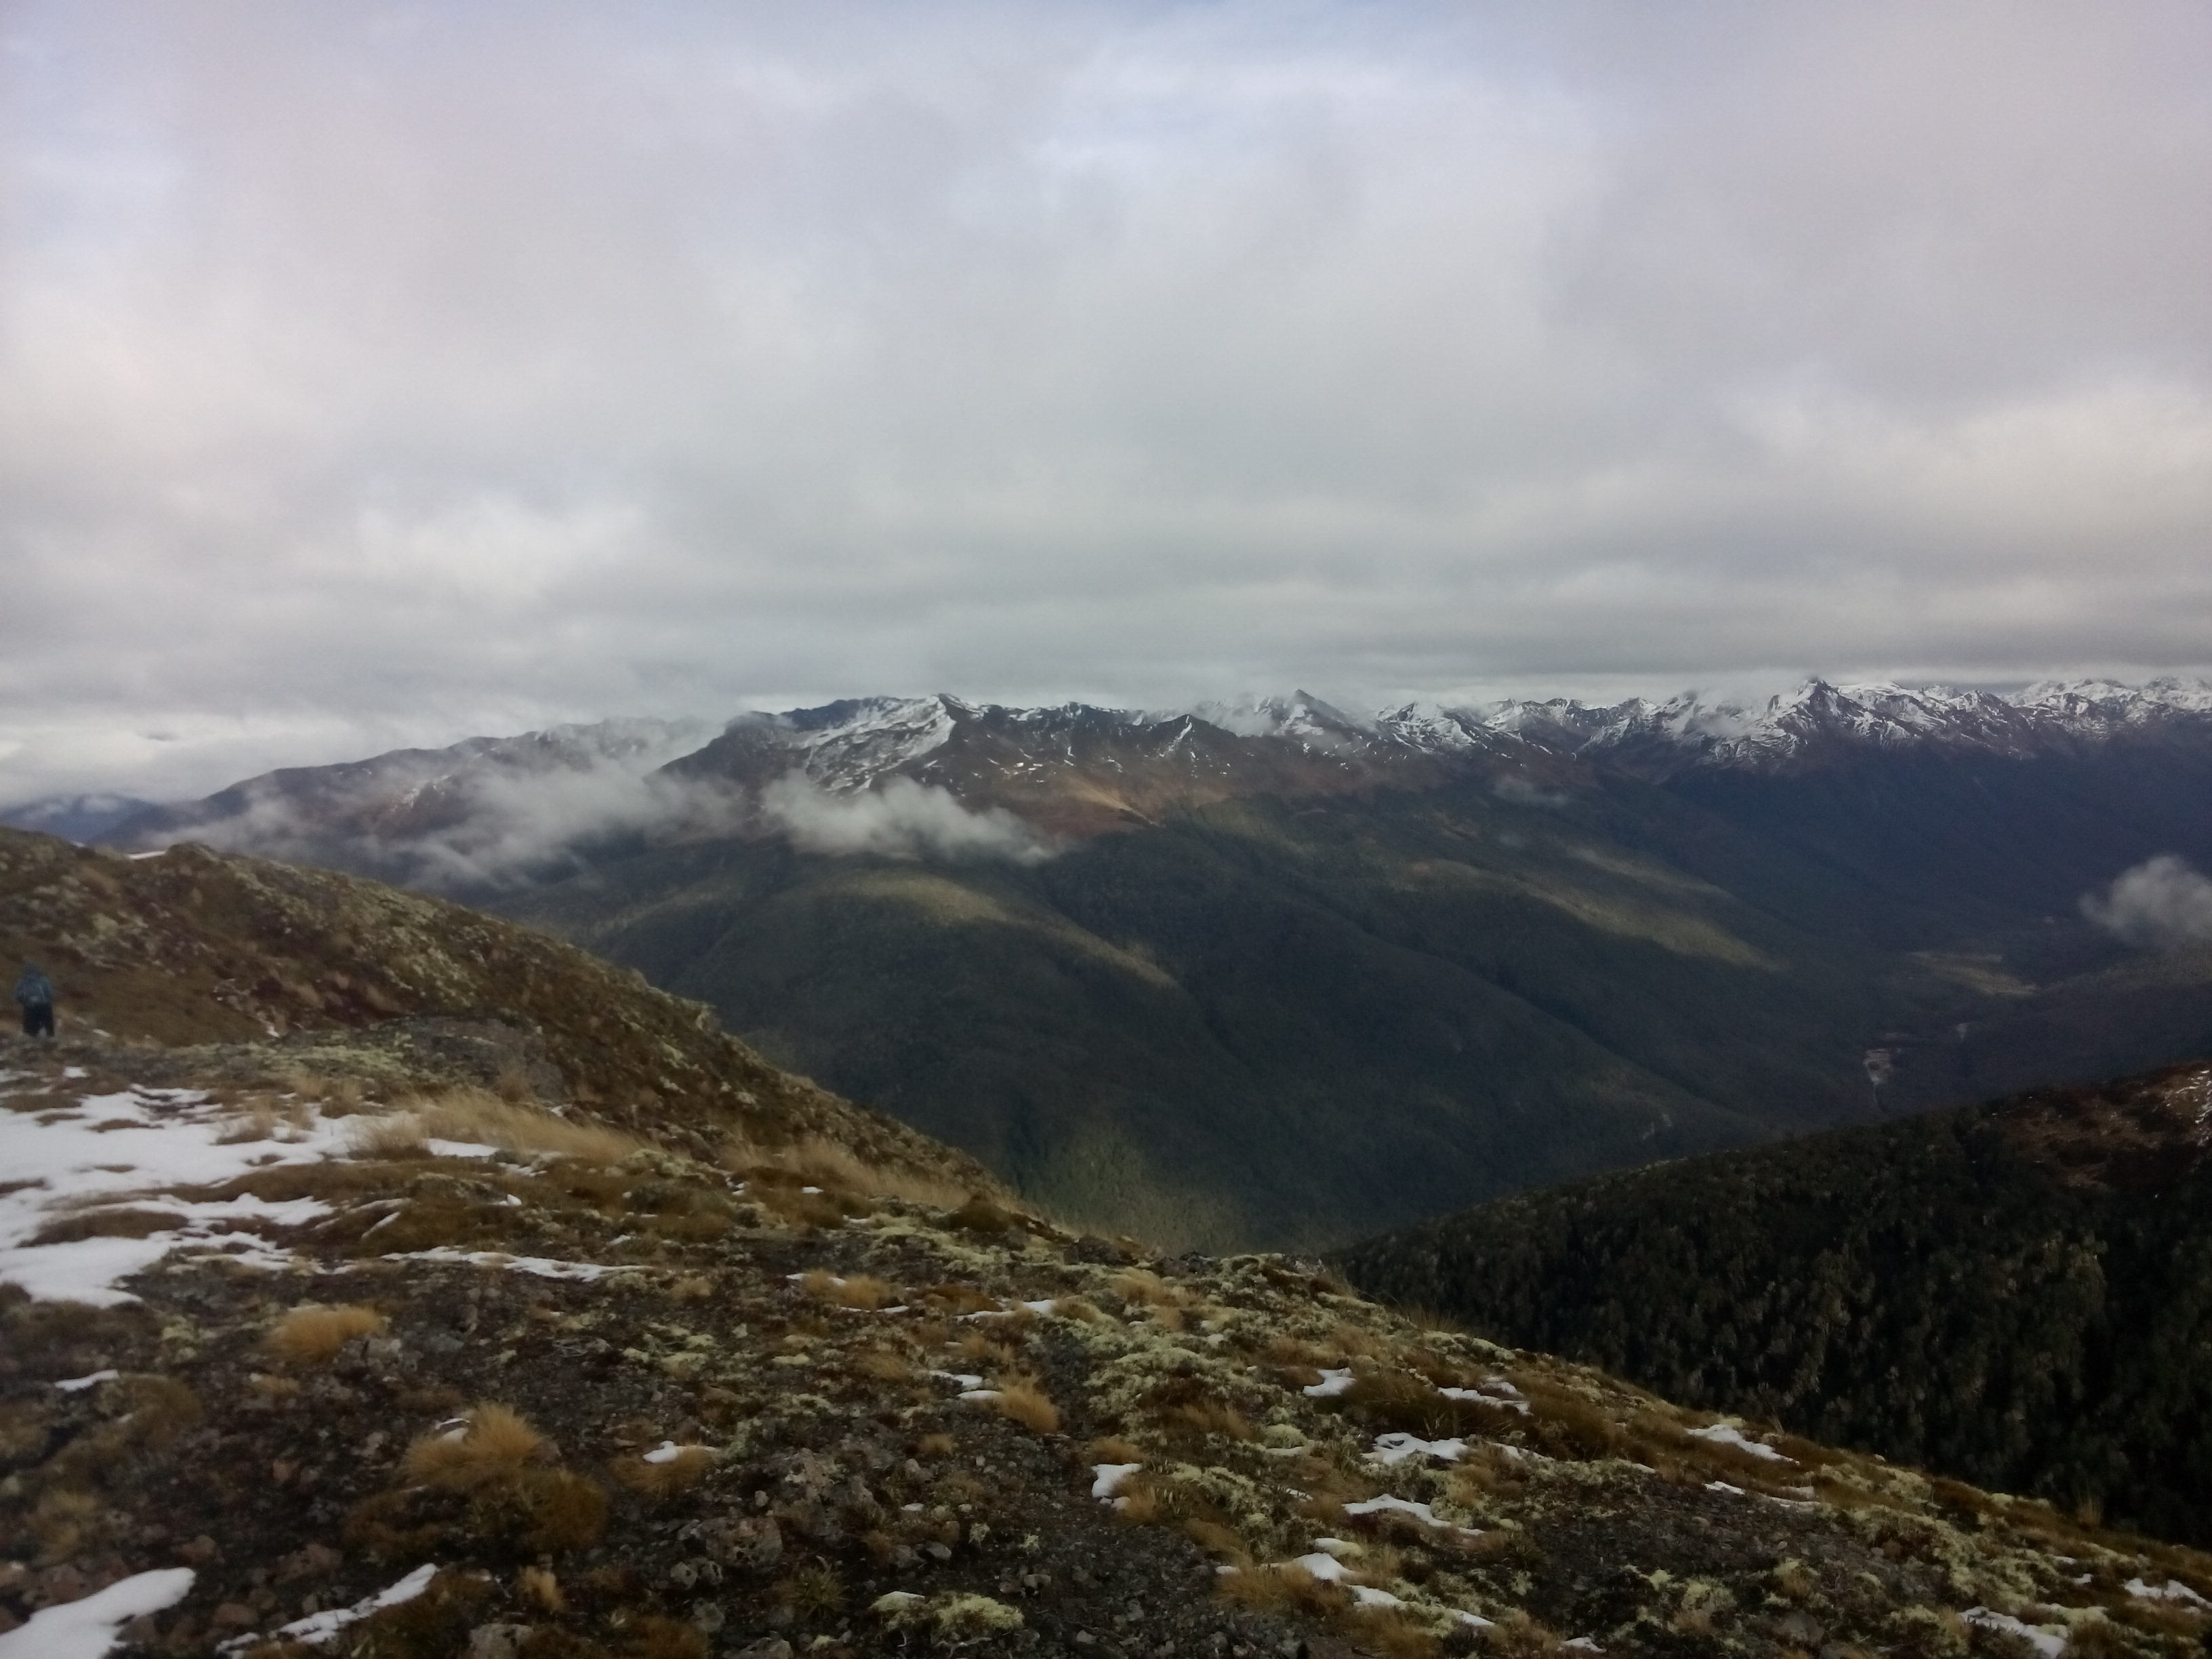
\includegraphics[width=8.5cm]{MtNorma28June2017Photo2}
% \end{flushright}
% \end{minipage}
% \end{figure}

\begin{flushright}
Robyn and Peter
\end{flushright}

\end{document}
